%======================================================================
\NEWSEC
%======================================================================

\subsection{\ssBlocks}

\begin{frame}[fragile,label=ss-blocks] 
\secframetitle{\ssBlocks}
\greenbf{Block objects represent blocks in the octree forest}

%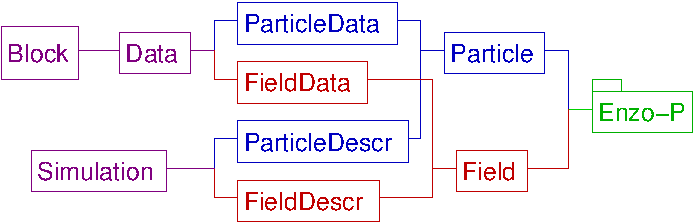
\includegraphics[width=2in]{data-classes.pdf}
\begin{tabbing}
xxxx\=xxxxxxxxxxxxxx\=\kill
\> \greencode{Data} \> \redit{Block data} \\
\> \greencode{Sync} \> \redit{Synchronization counters} \\
\> \greentext{state data} \> \redit{cycle, time, dt, etc.} \\
\> \greentext{face data} \> \redit{neighbor refinement levels} \\
\> \ \ \ \ \greenit{etc.}
\end{tabbing}
\vspace{-0.2in}
\begin{itemize}
\item Implemented as a \redit{chare array}
\item One \bluecode{EnzoBlock} object per octree forest node
\end{itemize}

\end{frame}

%----------------------------------------------------------------------

\begin{frame}[fragile,label=ss-blocks] 
\secframetitle{\ssBlocks}
\greenbf{\code{Data} objects contain numerical data associated with \code{Block}s}
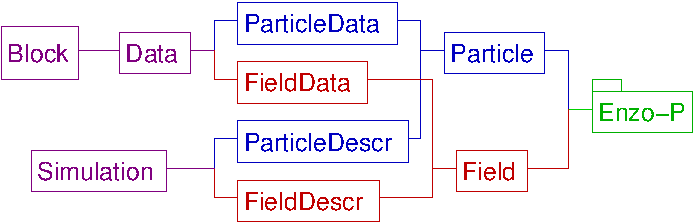
\includegraphics[width=2in]{data-classes.pdf}
\begin{tabbing}
xxxx\=xxxxxxxxxxxxxxxx\=\kill
\> \greencode{FieldBlock} \> \redit{Field (array) block data} \\
\> \greencode{ParticleBlock} \> \redit{Particle block data}
\end{tabbing}
\end{frame}
